\documentclass[journal]{IEEEtran}

\usepackage[UTF8,fontset=none,scheme=plain]{ctex}
\setmainfont{lmroman10-regular.otf}[
  BoldFont=lmroman10-bold.otf,
  ItalicFont=lmroman10-italic.otf,
  BoldItalicFont=lmroman10-bolditalic.otf]
\setCJKmainfont{Noto Serif CJK SC}
\setCJKsansfont{Noto Sans CJK SC}
\setCJKmonofont{Noto Sans Mono CJK SC}
\usepackage{amsmath}
\usepackage{amsfonts}
\usepackage{amssymb}
\usepackage{array}
\usepackage{booktabs}
\usepackage{graphicx}
\usepackage{tabularx}
\usepackage{url}
\def\SMUurlA{https://papers.nips.cc/paper_files/paper/2024/hash/7ede97c3e082c6df10a8d6103a2eebd2-Abstract-Conference.html}
\def\SMUurlB{https://doi.org/10.1109/DAC18074.2021.9586134}
\def\SMUurlC{https://doi.org/10.1109/AICAS59952.2024.10595882}
\def\SMUurlD{https://doi.org/10.1109/TC.2020.3027900}
\def\SMUurlE{https://doi.org/10.1109/TVLSI.2019.2950087}
\def\SMUurlF{https://doi.org/10.1109/ICFPT51103.2020.00014}
\def\SMUurlG{https://doi.org/10.1109/TCSII.2025.3585109}
\def\SMUurlH{https://doi.org/10.1109/MICRO56248.2022.00051}
\def\SMUurlI{https://doi.org/10.1109/ICFPT64416.2024.11113430}
\def\SMUurlJ{https://doi.org/10.1109/FPL57034.2022.00015}
\def\SMUurlK{https://doi.org/10.1109/TVLSI.2023.3305569}
\def\SMUurlL{https://doi.org/10.1145/3676536.3676743}
\def\SMUurlM{https://doi.org/10.1109/ICCAD57390.2023.10323651}
\def\SMUurlN{https://doi.org/10.1109/MDAT.2025.3527371}
\usepackage[hidelinks]{hyperref}
\setlength{\emergencystretch}{3em}
\renewcommand{\abstractname}{摘要}
\renewcommand{\IEEEkeywordsname}{关键词}
\renewcommand{\figurename}{图}
\renewcommand{\tablename}{表}
\renewcommand{\refname}{参考文献}

\newcolumntype{L}[1]{>{\raggedright\arraybackslash}m{#1}}
\newcolumntype{Y}{>{\raggedright\arraybackslash}X}

\title{Scalar SMU：面向RISC-V向量集群原生在线注意力的选择性递推加速}
\author{Xiaoteng Wang}

\begin{document}
\maketitle
\raggedbottom
\begin{abstract}
原生在线注意力通过增量处理分数块，持续更新归一化状态与输出。每个后续分块包含两类计算：更新运行最大值、归一化因子和重缩放权重的标量递推，以及作用于$D$个输出元素的向量更新。本文针对这两类计算的执行特征，在可编程RISC-V向量集群中设计选择性软硬件划分。集群内的标量在线合并单元（Scalar Online-Merge Unit，SMU）执行依赖状态的递推，现有Spatz/RVV数据通路执行规则输出更新。SMU采用阶段感知混合精度，并通过两条custom-2指令提供软件接口：OMCFG建立持久化上下文，OMERGE对一个后续分数块中的全部已配置查询行执行递推并返回完成状态。硬件管理交替使用的标量状态缓冲区，软件负责分块调度与输出向量管理。在四个原生在线注意力工作负载中，相对于采用相同RVV输出更新的标量软件基线，MMIO控制的选择性实现分别在递推、合并和Native Core计时范围内达到$8.524$--$17.784\times$、$4.144$--$6.275\times$和$1.066$--$1.157\times$的加速比。混合精度SMU的独立映射面积较旧版标量实现降低$27.6\%$。这些结果表明，状态递推专用化与现有向量资源复用能够共同支持在线注意力的选择性加速。
\end{abstract}
\begin{IEEEkeywords}
RISC-V；在线注意力；软硬件协同设计；领域专用加速；向量处理；混合精度计算；Softmax。
\end{IEEEkeywords}

\section{引言}
Transformer注意力将矩阵乘法与Softmax归一化相结合，是现代序列模型中的基本运算\cite{ref1}。在线归一化在分数到达时更新运行统计量\cite{ref2}。FlashAttention将这一思想应用于分块精确注意力，通过感知IO的执行方式降低中间数据的存储与访问开销\cite{ref3}。FlashAttention-2进一步改进GPU并行性和工作划分\cite{ref4}，FlashAttention-3引入异步调度与低精度执行\cite{ref5}。在可编程处理器上，分块执行同时形成了跨分块的状态递推依赖。

一次在线合并包含标量递推和向量更新。标量递推更新运行最大值与归一化因子，并生成两个输出重缩放权重。最大值选择、指数计算、累加和归一化构成一条异构依赖链，其运算数量相对于输出维度$D$保持固定。向量更新将两个权重独立应用于$D$个输出元素，具有规则的数据并行性。因此，一次合并同时包含$O(1)$的状态递推和$O(D)$的输出更新。

这一区别为软硬件划分提供了依据。专用递推单元能够集中处理状态依赖与非线性运算，现有向量处理器则适合执行规则的加权乘加。将两类计算分别映射到相应资源，可以在降低递推成本的同时复用向量数据通路；本文进一步通过完整卸载消融验证将输出更新保留在RVV一侧的必要性。

已有研究从算法、数值格式和硬件结构等方面优化在线归一化与非线性计算。Softermax将在线归一化与低精度算术结合，形成适合硬件实现的Softmax\cite{ref6}；SoftEx在RISC-V集群中加速Softmax和GELU\cite{ref7}；VEXP为Snitch RISC-V核增加近似指数运算，并评估其对Softmax和FlashAttention-2的影响\cite{ref8}。其他研究还探索了Softmax硬件与GELU计算之间的资源复用\cite{ref9}。RISC-V平台提供了带加速器接口的标量核\cite{ref10}、向量处理器\cite{ref11}和共享内存向量集群\cite{ref12}。TOP-V通过专用排序单元处理依赖密集的Top-K操作，展示了专用硬件与可编程向量执行相结合的设计方式\cite{ref13}。

本文在Spatz RISC-V向量集群中研究在线合并内部的选择性划分。集群内的标量在线合并单元执行状态递推，现有RISC-V向量（RVV）数据通路执行$D$维输出更新。SMU按照计算阶段采用固定的混合精度，以FP32作为内存接口格式，在内部使用FP16、定点查表和Q16.32累加。

软件通过OMCFG和OMERGE两条custom-2指令控制SMU。OMCFG配置状态数组、块内统计量、权重数组的TCDM地址与查询行数，随后提交上下文。OMERGE对一个后续分数块处理全部已配置查询行，并返回完成状态。硬件管理标量状态缓冲区的交替选择，软件负责分块调度、输出缓冲区指针和RVV更新。该接口将有状态递推接入RISC-V核的加速器请求通路，并复用现有向量指令完成输出更新。

在四个原生在线注意力工作负载中，选择性递推卸载相对于共享RVV输出例程的软件基线，最高实现$17.8\times$的递推加速和$1.16\times$的Native Core加速。独立综合显示，混合精度SMU的映射面积较旧版标量单元降低$27.6\%$。指令接口进一步降低了逐次递推调用和一次性上下文配置的开销。

本文的主要贡献如下：
\begin{enumerate}
\item 刻画在线合并中状态递推与输出更新的执行差异，提出并评估选择性软硬件划分：SMU执行依赖状态的标量递推，现有RVV数据通路执行规则的$D$维输出更新。
\item 定义面向这一划分的RISC-V编程接口。OMCFG建立持久化上下文，OMERGE执行分块递推；硬件管理交替标量状态并将完成响应返回发起核，软件管理输出缓冲区与向量执行。
\item 实现阶段感知混合精度SMU，将FP16、定点非线性近似和Q16.32累加应用于相应计算阶段，并评估数值一致性、映射面积和时序特征。
\end{enumerate}

\section{原生在线注意力与设计动机}
\subsection{原生在线注意力}
全文中，$N$表示配置的查询行数，$B$表示键分块大小，$D$表示输出向量长度，$t$表示分块索引。本文评估的工作负载采用相同的查询与键序列长度，且$N$可被$B$整除，因此分块数量为$T=N/B$。权重下标tile表示对应的分块贡献，撇号表示合并后的状态，帽号表示经过硬件阶段转换后的数值。

在QI.F定点格式中，$I$表示整数幅值位数，$F$表示小数位数；有符号格式额外包含一个符号位。

注意力根据查询与键之间的相似度聚合值向量。在线注意力逐块处理分数，增量维护归一化状态和输出，将概率计算与输出累加组织为分块执行流程。在线归一化是在线Softmax\cite{ref2}和感知IO的精确注意力\cite{ref3}的基础。

对于一个查询行，令$s_i$表示已处理位置$i$的分数，$\mathbf v_i$表示对应的值向量。累积状态为$(m,l,\mathbf O)$，满足以下不变量：
\begin{equation}
\begin{gathered}
 m=\max_i s_i,\\
 l=\sum_i\exp(s_i-m),\\
 \mathbf O=\frac{1}{l}\sum_i\exp(s_i-m)\mathbf v_i.
\end{gathered}
 \label{eq:invariant}
\end{equation}
其中，$l$为相对于运行最大值$m$的归一化因子，$\mathbf O\in\mathbb R^D$为归一化部分输出。新的分数块提供状态$(m_t,l_t,\mathbf O_t)$。

两组状态通过以下标量递推合并：
\begin{equation}
\begin{aligned}
 m'&=\max(m,m_t),\\
 l'&=l\exp(m-m')+l_t\exp(m_t-m'),\\
 w_{\mathrm{old}}&=\frac{l\exp(m-m')}{l'},\\
 w_{\mathrm{tile}}&=\frac{l_t\exp(m_t-m')}{l'}.
\end{aligned}\label{eq:recurrence}
\end{equation}
向量输出更新为：
\begin{equation}
 \mathbf O'=w_{\mathrm{old}}\mathbf O+w_{\mathrm{tile}}\mathbf O_t.
 \label{eq:vector}
\end{equation}
首个分块初始化运行状态，每个后续分块执行式\eqref{eq:recurrence}和式\eqref{eq:vector}。输出在每次合并后保持归一化，最终结果由最后一次合并直接给出。

\subsection{执行特征}
图\ref{fig:split}将在线合并分解为状态递推和向量更新。递推更新$m$、$l$并生成两个重缩放权重，向量通路将这些权重应用于$D$个输出元素。

标量递推中的最大值选择、指数重缩放、累加和归一化形成异构依赖链。运行状态在分块之间传递，当前分块的计算结果成为后续分块的输入。对每个查询行，递推执行固定数量的运算，其工作量相对于$D$为$O(1)$。

各输出元素按下式更新：
\begin{equation}
 O'[j]=w_{\mathrm{old}}O[j]+w_{\mathrm{tile}}O_t[j],\qquad 0\le j<D.
 \label{eq:element}
\end{equation}
全部$D$个元素共享相同的两个权重，并可独立更新。该过程是规则的浮点加权乘加循环，工作量为$O(D)$，适合映射到现有RVV执行资源。

因此，本文将状态递推映射到SMU，将分数生成、块内状态构建和输出更新保留在可编程通路。对于配置了$N$行的分块合并，SMU依次执行各行的标量递推，RVV将对应权重应用于每行的$D$个输出元素。
\begin{figure*}[t]
\centering
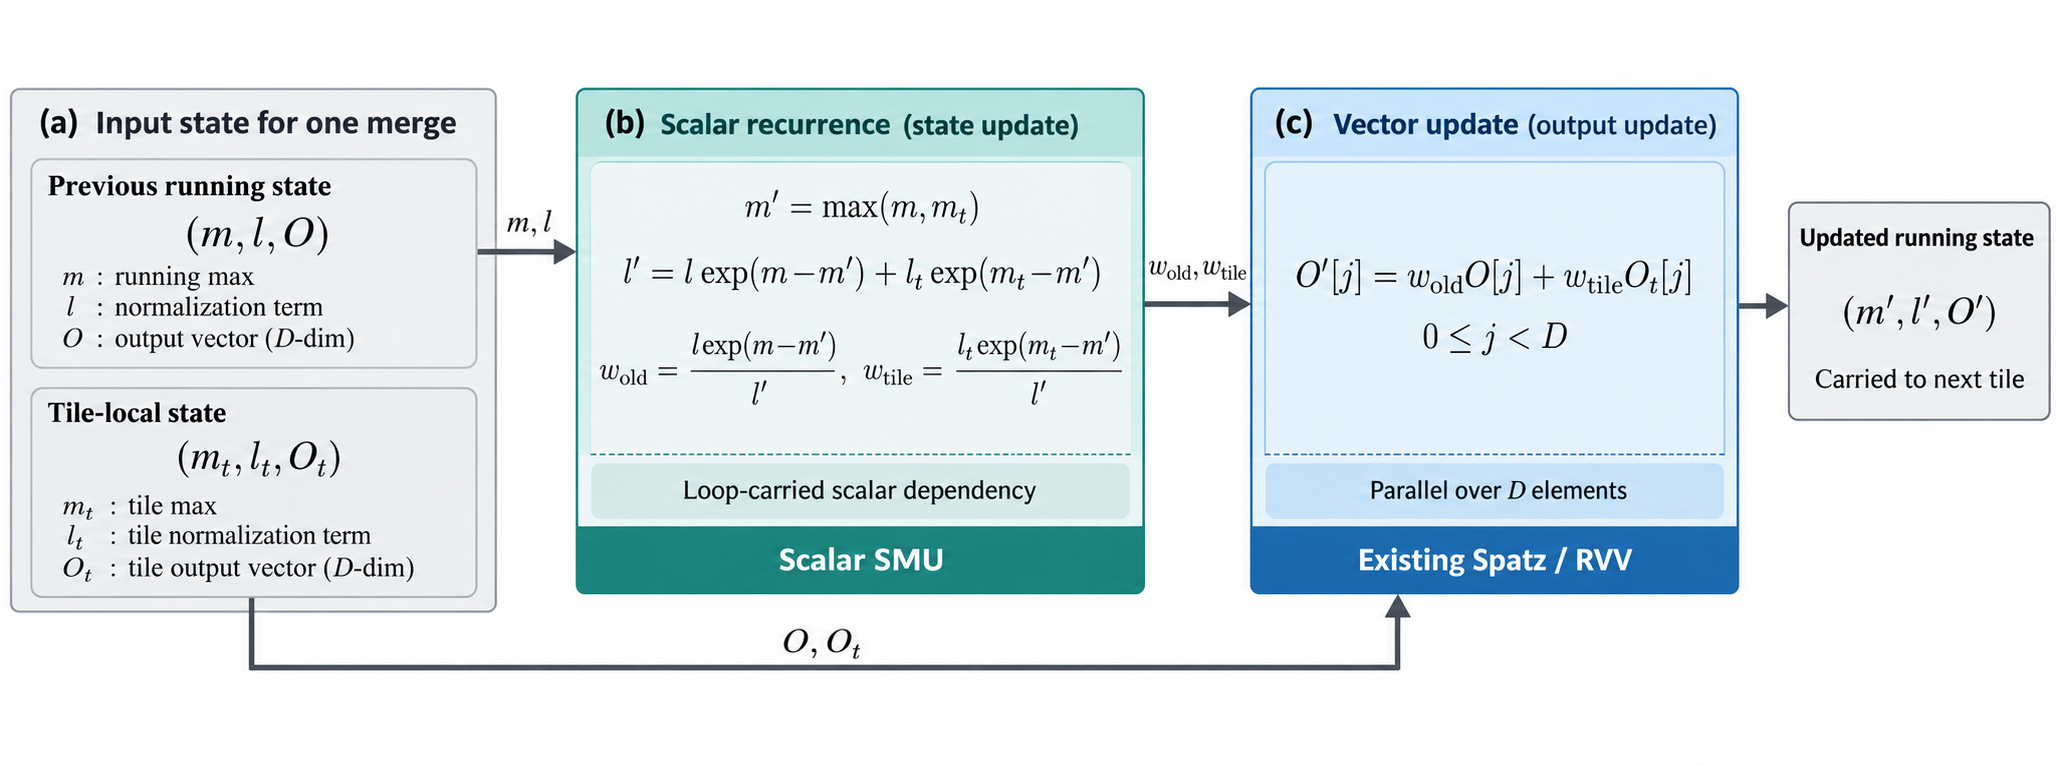
\includegraphics[width=\textwidth,trim=0 58 0 0,clip]{./figure/fig1.png}
\caption{原生在线注意力合并的执行分解。SMU更新运行最大值与归一化因子，并生成两个标量重缩放权重；现有Spatz/RVV数据通路执行$D$维输出更新。}
\label{fig:split}
\end{figure*}

\subsection{设计目标}
上述执行特征引出三个设计目标。

第一，选择性专用化。使用专用硬件处理递推依赖链，并复用Spatz/RVV执行规则输出更新，使状态递推加速与现有向量资源复用相结合。

第二，轻量化递推实现。按照各计算阶段的数值范围和精度要求分配格式，将混合精度应用于最大值、非线性近似、归一化累加和权重生成。

第三，支持跨分块重复调用。软件一次建立工作负载上下文，随后逐块调用递推；硬件管理交替使用的标量状态，软件负责向量输出与分块调度。

最终映射由集群内SMU、现有Spatz/RVV数据通路和共享TCDM共同组成。SMU执行递推，RVV执行输出更新，适配器管理标量状态的A/B选择位。

\section{架构与软硬件协同设计}
\subsection{系统概览与软硬件划分}
图\ref{fig:system}展示SMU在Spatz向量集群中的集成方式\cite{ref12}。Snitch标量核、Spatz/RVV数据通路和SMU通过紧耦合数据存储器（TCDM）交换数据。默认配置的TCDM容量为128 KiB，分为16个存储体。

OMERGE命令经过Snitch译码、各核加速器解复用器、集群发射仲裁器和SMU适配器。仲裁器记录发起核，响应解复用器将完成响应返回对应核。Spatz/RVV指令通过直接向量通路进入向量处理器。

SMU作为独立TCDM请求端读取标量操作数，并写入更新状态与权重。该设计保留Spatz/RVV的通道、浮点单元、向量寄存器文件及现有指令语义。RVV例程通过共享内存读取权重，使用现有向量资源执行式\eqref{eq:vector}和式\eqref{eq:element}。

Native Core计时范围从已驻留内存的Q/K/V数据开始，覆盖分数块计算、局部状态构建、首块初始化、后续合并、RVV输出更新和最终输出复制。内存分配、输入生成、诊断、Q/K/V加载和线性投影在该计时范围之前完成。

首块将$(m_t,l_t,\mathbf O_t)$写入运行状态。随后，每条OMERGE对一个分数块中的全部已配置$N$行执行递推。对每行，SMU读取当前$m$、$l$与块内$m_t$、$l_t$，将更新后的$m$、$l$写入目标标量缓冲区，并将两个重缩放权重写入TCDM。全部行完成后，适配器返回状态；发起核接收成功响应后，A/B选择位翻转。Spatz/RVV随后读取权重并更新输出，软件推进输出缓冲区指针。

这一划分使SMU专注于标量递推，软件和Spatz/RVV承担分数生成、局部状态构建、首块初始化、输出寻址、向量更新和最终复制。
\begin{figure}[t]
\centering
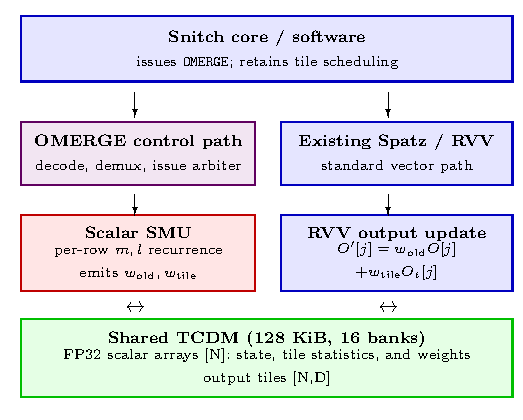
\includegraphics[width=\columnwidth]{./figure/fig2_v4.pdf}
\caption{系统集成与软硬件划分。Snitch核通过加速器译码、解复用器和集群发射仲裁器向SMU提交OMERGE，适配器将完成状态返回发起核。Spatz/RVV通过现有向量通路执行输出更新，两类计算通过共享TCDM交换状态、权重和输出数据。}
\label{fig:system}
\end{figure}

\subsection{阶段感知混合精度SMU}
SMU采用设计时固定的阶段精度分配，计算式\eqref{eq:recurrence}的阶段量化近似，如图\ref{fig:precision}所示。FP32用于内存接口，FP16用于最大值及部分转换边界，定点查表用于非线性近似，Q16.32用于归一化累加。

用$\operatorname{RNE}_{16}(\cdot)$表示采用舍入到最近偶数方式转换至FP16。输入最大值及其差值按以下过程计算：
\begin{equation}
\begin{aligned}
 \hat m&=\operatorname{RNE}_{16}(m),&
 \hat m_t&=\operatorname{RNE}_{16}(m_t),\\
 \hat m'&=\max(\hat m,\hat m_t),\\
 \hat\Delta_{\mathrm{old}}&=\operatorname{RNE}_{16}(\hat m-\hat m'),\\
 \hat\Delta_{\mathrm{tile}}&=\operatorname{RNE}_{16}(\hat m_t-\hat m').
\end{aligned}\label{eq:max}
\end{equation}
EXP阶段采用含256项的有符号Q1.14查找表，其索引为：
\begin{equation}
 i(\Delta)=\left\lfloor(\Delta+8)\cdot32\right\rfloor,
 \qquad \Delta\in[-8,0).
 \label{eq:exp}
\end{equation}
表项编码各区间中心的指数近似值，硬件直接读取对应表项。满足$\Delta\ge0$的贡献使用单位缩放因子；$\Delta\in[-8,0)$的贡献通过LUT获得缩放因子，其中$\Delta=-8$访问LUT[0]；$\Delta<-8$时缩放因子置零。转换后的两个最大值相等时，两条通路均使用单位值。所得缩放因子分别记为$\hat s_{\mathrm{old}}$和$\hat s_{\mathrm{tile}}$。

SMU将$l$和$l_t$从FP32转换为无符号Q16.32，得到$\hat l$与$\hat l_t$，并计算：
\begin{equation}
 \hat l'=\hat l\hat s_{\mathrm{old}}+\hat l_t\hat s_{\mathrm{tile}}.
 \label{eq:sum}
\end{equation}
累加结果保持为Q16.32格式。计算倒数前，分母经过FP16舍入，并转换为倒数计算所用的规范化表示。令规范化分母为$\hat x=2^{e-127}(1+\mu)$，其中$e$为带偏置指数，$\mu$为尾数小数部分。倒数近似采用查表与线性插值：
\begin{equation}
\begin{aligned}
 \frac{1}{\hat x}&\approx2^{127-e}\left[L_j+(L_{j+1}-L_j)f_j\right],\\
 j&=\lfloor256\mu\rfloor,\qquad f_j=256\mu-j.
\end{aligned}\label{eq:reciprocal}
\end{equation}
其中，$L_j$为$1/(1+j/256)$的无符号Q1.15编码，$f_j$由尾数低15位承载。

所得倒数用于缩放分子。缩放分子经过FP16舍入边界，并在生成权重前转回Q16.32。一个共享的$48\times16$乘法器依次生成旧状态权重与分块权重。

该数据通路处理FP16转换后为正有限值的分母，定点中间结果保持在Q16.32表示范围内。定向模型测试覆盖零分子、次正规分母和最大有限FP16分母。阶段量化误差来自EXP截断、查表量化和FP16舍入。

更新后的最大值与归一化因子转换为FP32并写回TCDM，其中最大值经过FP16舍入，归一化因子采用Q16.32累加。合并权重经FP16舍入后转换为FP32，供Spatz/RVV执行输出更新。由此，内存接口采用FP32，内部递推按阶段使用FP16与定点格式。
\begin{figure}[t]
\centering
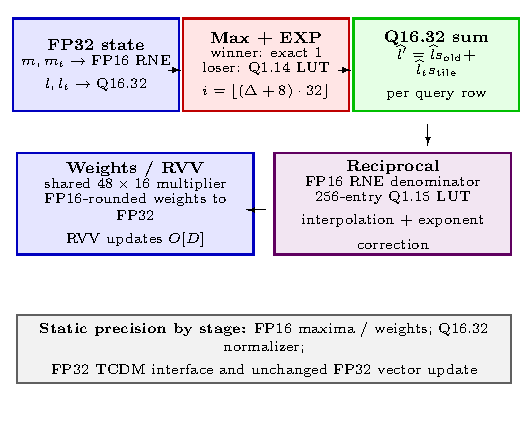
\includegraphics[width=\columnwidth]{./figure/fig3_v4.pdf}
\caption{阶段感知混合精度SMU数据通路。图中展示FP32输入接口、FP16最大值与转换边界、Q16.32归一化累加、EXP查表、插值倒数计算，以及供RVV输出更新使用的合并权重。}
\label{fig:precision}
\end{figure}

\subsection{RISC-V指令接口}
编程模型将持久化上下文配置与逐次递推调用组织为两类操作。OMCFG与OMERGE采用RISC-V为实现相关扩展保留的custom-2操作码空间\cite{ref14}，并通过Snitch加速器请求通路访问SMU。现有RVV编码与向量指令语义保持一致。

表\ref{tab:isa}给出指令格式及其作用。
\begin{table*}[t]\centering\small
\caption{Custom-2指令格式及其作用。}
\label{tab:isa}
\begin{tabularx}{\linewidth}{lYYY}
\toprule
指令 & 编码字段 & 操作数字段 & 作用\\
\midrule
OMERGE & R型；opcode=0x5B；funct7=0000011；funct3=000 & rs1=rs2=x0；rd接收完成状态 & 对一个分数块中的全部配置行执行递推，通过TCDM更新标量状态与权重\\
OMCFG & 类I型；opcode=0x5B；funct3=001 & imm12选择配置标识；rs1提供数值；rd=x0 & 写入持久化上下文字段，或通过INIT提交上下文\\
\bottomrule
\end{tabularx}
\end{table*}
两条指令通过固定功能位区分配置与执行操作。表\ref{tab:decode}给出译码掩码、匹配值和机器字表达式。
\begin{table}[t]\centering\small
\caption{OMERGE与OMCFG的译码模式。指令字与掩码按位与后等于匹配值时，译码器识别对应操作。}
\label{tab:decode}
\begin{tabularx}{\linewidth}{lllY}
\toprule
指令 & 掩码 & 匹配值 & 机器字表达式\\
\midrule
OMERGE & 0xFFFFF07F & 0x0600005B & \texttt{0x0600005B | (rd << 7)}\\
OMCFG & 0x00007FFF & 0x0000105B & \texttt{(cfg\_id << 20) | (rs1 << 15) | 0x0000105B}\\
\bottomrule
\end{tabularx}
\end{table}

OMERGE对一个后续分数块中的全部已配置$N$行执行标量递推。其rs1与rs2字段均指定x0，操作数通过持久化上下文中的TCDM地址读取。适配器采用Mixed Scalar模式，与MMIO控制通路使用相同算术，$D$维输出由现有RVV例程更新。

rd字段指定完成状态目标寄存器。软件通过非零rd接收并检查状态；rd=x0时，返回状态被丢弃。发射时，Snitch在加速器记分牌中预留目标寄存器，并通过各核解复用器与集群仲裁器转发指令及请求标识。

适配器以一条在途命令为粒度工作，依次经过IDLE、START、WAIT和RESP状态。WAIT阶段等待SMU报告DONE或ERROR，RESP阶段将请求标识和状态返回发起核。核接收响应后写入rd，并清除对应的记分牌条目。零状态表示成功，非零状态表示错误。

递推/控制计时窗口覆盖指令发射、SMU执行、响应提交和软件状态消费。OMERGE接口比较采用相同的SMU算术与RVV更新例程，评估每个非首块递推的调用开销。

\subsection{通过OMCFG建立持久化上下文}
状态数组地址与工作负载参数在连续分块之间保持稳定。OMCFG在执行前建立持久化上下文，随后每个后续分数块通过一次OMERGE调用处理全部已配置查询行。

OMCFG与OMERGE共享custom-2操作码；其中OMCFG使用funct3=001。类I型编码通过imm12选择配置字段，通过rs1提供字段值，rd固定为x0。适配器在自身及SMU引擎均空闲时接受配置命令。

配置标识0x000--0x008对应九个必需字段，指定两组运行状态数组、块内统计量数组、两个权重数组的TCDM基址和查询行数$N$。标识0x009选择CTRL/INIT操作，其数值位0置位时提交上下文并复位A/B选择位。
\begin{table*}[t]\centering\small
\caption{OMCFG配置标识与字段映射。}
\label{tab:cfg}
\begin{tabularx}{\linewidth}{lllY}
\toprule
cfg\_id & 字段 & 数值类型 & 用途\\
\midrule
0x000 & A\_M & TCDM地址 & A缓冲区的运行最大值数组\\
0x001 & A\_L & TCDM地址 & A缓冲区的运行归一化因子数组\\
0x002 & B\_M & TCDM地址 & B缓冲区的运行最大值数组\\
0x003 & B\_L & TCDM地址 & B缓冲区的运行归一化因子数组\\
0x004 & TILE\_M & TCDM地址 & 块内最大值数组\\
0x005 & TILE\_L & TCDM地址 & 块内归一化因子数组\\
0x006 & WEIGHT\_OLD & TCDM地址 & 旧状态重缩放权重数组\\
0x007 & WEIGHT\_TILE & TCDM地址 & 分块重缩放权重数组\\
0x008 & N & 查询行数 & 每条OMERGE处理的行数\\
0x009 & CTRL/INIT & 位0置位 & 提交上下文并复位选择位\\
0x00A--0xFFF & 保留 & --- & 访问后上下文进入待初始化状态\\
\bottomrule
\end{tabularx}
\end{table*}
每个地址指向逐行FP32数组，第$r$行的地址为：
\[
 \operatorname{scalar\_addr}(\mathrm{base},r)=\mathrm{base}+4r.
\]

OMCFG与MMIO访问同一组持久化配置寄存器，软件可通过MMIO读取配置值。适配器记录九个必需字段的写入状态；全部字段准备完成后，INIT提交上下文并将选择位复位为零。字段重写后，软件再次执行INIT以提交更新后的上下文。

OMCFG负责标量状态、统计量、权重地址与查询行数配置。输出维度$D$、块大小、输出地址和步长由软件及RVV例程管理。适配器固定采用Mixed Scalar模式，内部相应字段设置为$D=1$和零步长。保留标识使上下文进入待初始化状态，软件通过完整INIT恢复就绪状态。

\subsection{调用序列与状态管理}
TCDM中保存两组标量运行状态：
\[
 A=(A_m,A_l),\qquad B=(B_m,B_l).
\]
每组为全部$N$个查询行保存FP32最大值和归一化因子。一个硬件选择位决定当前源缓冲区与目标缓冲区：选择位为零时读取A并写入B，选择位为一时读取B并写入A。

软件首先计算首块，将初始标量状态写入A，并初始化输出缓冲区。随后写入九个配置字段并提交INIT，使选择位复位为零。第一次后续合并读取A、写入B，此后的合并交替改变方向。

发起核接收成功响应后，适配器提交选择位转换。配置尚待提交或SMU报告错误时，命令返回非零状态，选择位保持当前值；配置检查在引擎启动前完成。

本文采用单控制核、单活动上下文的执行方式。硬件管理逐行$m/l$状态的A/B选择位，软件管理分块地址与两个$D$维输出缓冲区指针。每次递推成功完成后，软件读取返回状态，调用RVV例程更新输出，并交换输出缓冲区指针。
\begin{figure*}[t]
\centering
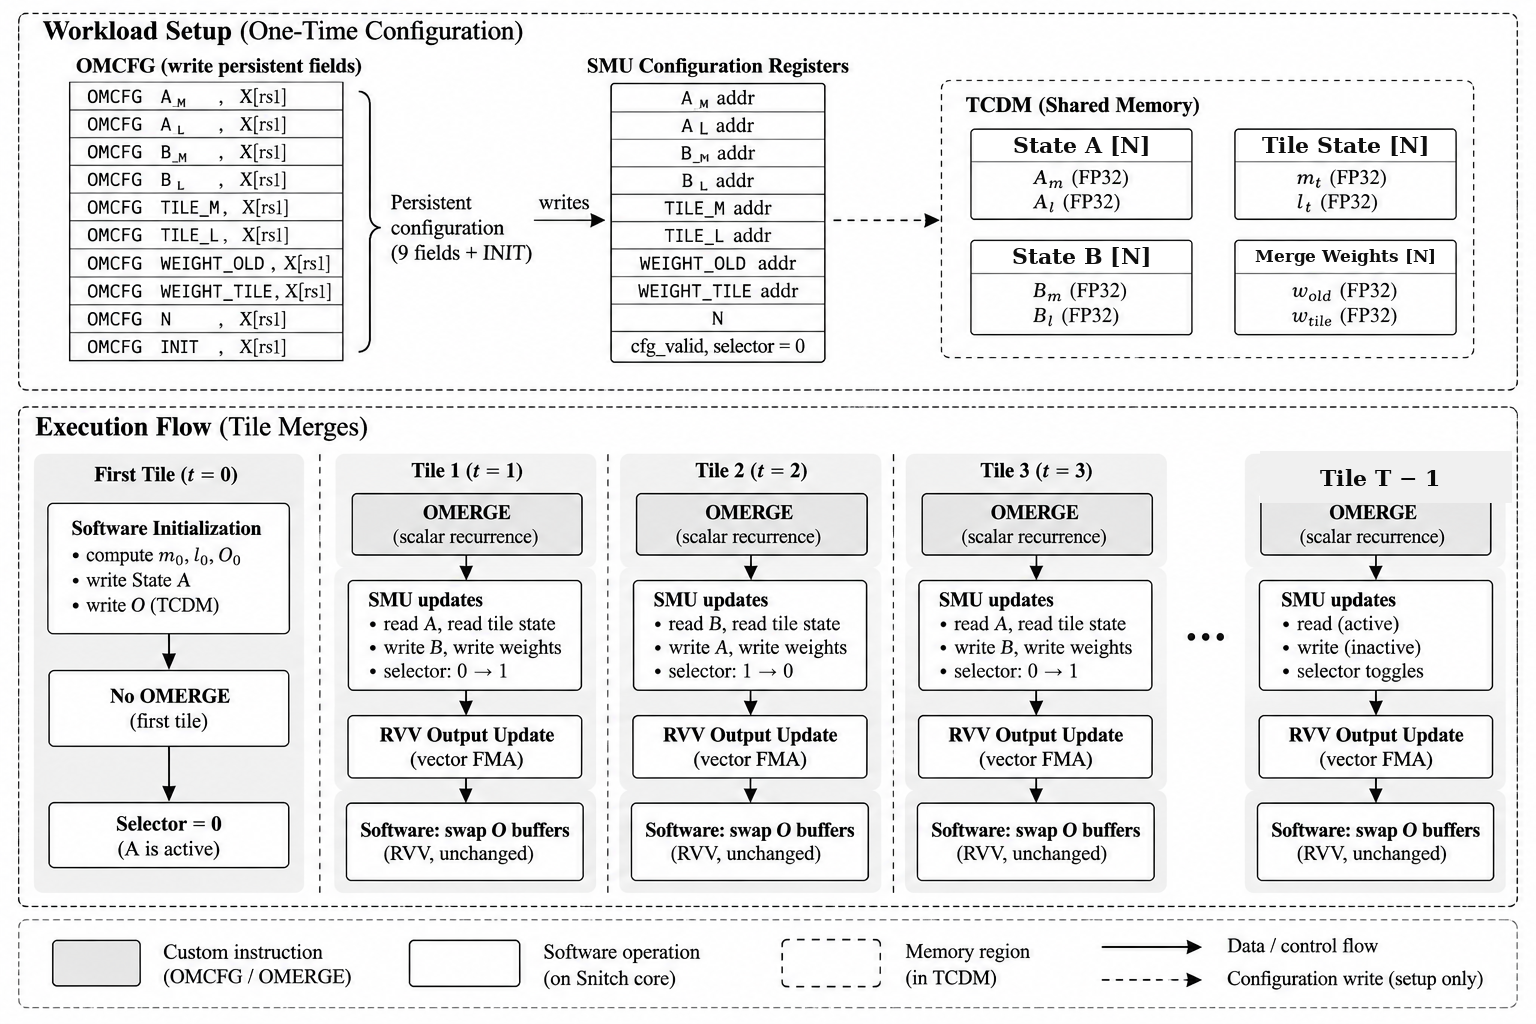
\includegraphics[width=\textwidth]{./figure/fig4_v4.png}
\caption{OMCFG/OMERGE编程模型。一次性配置建立持久化标量上下文。每个后续分数块通过一条OMERGE处理全部已配置查询行，随后执行RVV输出更新。配置指令将上下文地址写入寄存器，SMU通过TCDM访问状态与权重。硬件管理标量状态选择位，软件管理输出缓冲区。}
\label{fig:program}
\end{figure*}

\section{评估}
\subsection{实验设置与测量范围}
性能评估采用Spatz RISC-V向量集群的周期级仿真。模型由Verilator 5.034构建，使用默认集群配置，其中TCDM容量为128 KiB，分为16个存储体。各阶段通过周期计数器测量，每组匹配比较采用相同的集群配置与软件工具链。

N8/D32和N16/D64用于主要接口比较，N24/D64和N16/D128用于考察序列长度与输出维度变化。所有原生注意力案例采用块大小$B=4$和种子1。接口实验采用单控制核、单活动上下文。

首块初始化运行状态，每个查询行执行$T-1$次后续合并。四个工作负载分别包含1、3、5和3次后续分块合并。每个后续分数块通过一条OMERGE处理全部已配置$N$行。

性能评估采用三个逐级扩大的计时范围：递推窗口覆盖状态与权重生成，MMIO控制通路同时计入配置、启动、轮询和SMU执行；合并窗口进一步计入RVV输出更新与合并调度；Native Core从已驻留内存的Q/K/V开始，覆盖分数块计算、局部状态构建、首块初始化、后续合并、输出更新与最终输出处理。

评估按研究目标组织为三组匹配比较。算术卸载组比较标量软件递推加RVV的B2R基线与MMIO控制的SMU加相同RVV更新；逐次调用组比较MMIO与OMERGE；配置组在采用OMERGE执行的条件下比较MMIO与OMCFG。

B2R在标量软件中计算式\eqref{eq:recurrence}，并与SMU通路共享RVV输出例程。软件与SMU分别采用各自的内部数值格式，因此该比较体现硬件专用化与阶段精度分配的联合效果。各实验组分别使用匹配的基线与实现版本。

周期级仿真使用固定输入。接口实验对每个通路与形状执行一次正式测量，加速比定义为匹配基线与目标实现的周期数比值。

\subsection{原生在线注意力性能}
原生比较保持RVV输出更新一致，评估选择性递推卸载的效果。图\ref{fig:speedup}汇总三个计时范围的加速比。

在N8/D32中，递推由12,368降至1,451周期，加速比为$8.524\times$；合并由13,204降至2,318周期，加速比为$5.696\times$；Native Core由85,262降至73,706周期，加速比为$1.157\times$，周期数降低$13.554\%$。

在N16/D64中，递推由68,994降至4,926周期，加速比为$14.006\times$；合并由77,037降至13,060周期，加速比为$5.899\times$；Native Core由571,374降至507,918周期，加速比为$1.125\times$，周期数降低$11.106\%$。

N24/D64在递推、合并和Native Core范围内分别达到$17.784\times$、$6.275\times$和$1.140\times$加速。N16/D128分别达到$13.737\times$、$4.144\times$和$1.066\times$加速。

随着计时范围扩大，分数构建、块内状态生成和RVV输出更新逐步计入总周期。这些计算占据更大比例，使递推、合并和Native Core呈现依次递减的加速比。
\begin{figure*}[t]
\centering
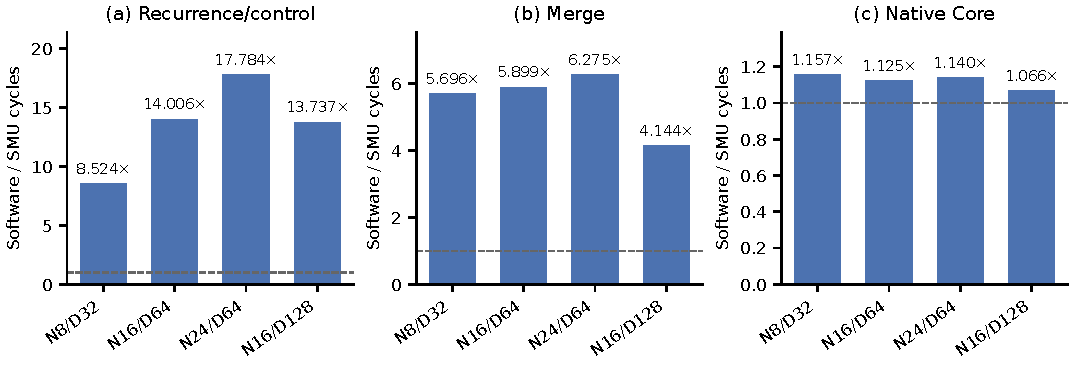
\includegraphics[width=\textwidth]{./figure/fig5.pdf}
\caption{原生在线注意力在三个计时范围内的加速比，定义为匹配软件基线与SMU通路的周期数比值。MMIO控制的递推窗口计入配置、启动、轮询和SMU执行。各工作负载采用块大小$B=4$，三个子图分别使用与其加速比范围对应的纵轴刻度。}
\label{fig:speedup}
\end{figure*}

\subsection{数值一致性与SMU硬件成本}
数值评估以B2R软件输出为参照，使用float64计算两条通路FP32存储结果之间的MAE与相对误差$\sum|\Delta|/\sum|O|$。四个原生工作负载的MAE为$2.8\times10^{-4}$--$5.6\times10^{-4}$，相对误差为$0.49\%$--$0.71\%$，输出均为有限值。

独立数值扫描进一步评估倒数近似和整体阶段量化误差。穷举31,743个正有限FP16分母得到最大倒数相对误差$6.70\times10^{-5}$。

主机模型的正式扫描覆盖长度128、256、512和1024，维度64和128的随机分数与单头Q/K/V案例，共16种组合，块大小为32，基础种子为20260823。倒数查表参数的扩展扫描显示，倒数替代实现相对于除法实现的最大相对误差为$0.11\%$，优化实现相对于FP32参考实现的最大相对误差为$1.5\%$。

硬件成本通过独立Yosys/ABC综合评估，采用Nangate45典型工艺库，面积以该Liberty库的单元面积单位报告。Mixed+Division的映射面积为52,000，较旧版标量设计的72,399降低$28.2\%$；Mixed+Reciprocal的映射面积为52,408，较旧版降低$27.6\%$，较Mixed+Division增加$0.8\%$。
\begin{table*}[t]\centering\small
\caption{与软件递推的数值一致性及独立SMU综合面积。}
\label{tab:accuracy}
(a) 与B2R软件输出的一致性\par\medskip
\begin{tabular}{lrr}
\toprule
工作负载 & MAE & 相对误差\\
\midrule
N8/D32 & $2.79\times10^{-4}$ & $0.49\%$\\
N16/D64 & $4.67\times10^{-4}$ & $0.71\%$\\
N24/D64 & $3.74\times10^{-4}$ & $0.61\%$\\
N16/D128 & $5.63\times10^{-4}$ & $0.52\%$\\
\bottomrule
\end{tabular}\par\medskip
(b) 独立SMU综合结果\par\medskip
\begin{tabular}{lrr}
\toprule
设计 & 映射面积（库单位） & 面积降幅\\
\midrule
旧版标量设计 & 72,399 & ---\\
Mixed+Division & 52,000 & $28.2\%$\\
Mixed+Reciprocal & 52,408 & $27.6\%$\\
\bottomrule
\end{tabular}
\end{table*}

\subsection{软硬件划分消融}
划分消融比较两种输出更新方式。选择性设计使用SMU执行标量递推、使用RVV执行$D$维输出更新；Full SMU将两部分均放入加速器。该消融测量合并微内核周期，两个设计取自同一消融实现版本；表\ref{tab:accuracy}(b)的混合精度综合结果来自独立的实现版本。
\begin{table}[t]\centering
\caption{选择性卸载与完整卸载的合并微内核周期。}
\label{tab:ablation}
\begin{tabular}{lrrr}
\toprule
工作负载 & 选择性设计周期 & Full SMU周期 & 完整/选择性\\
\midrule
N12/D64 & 4,128 & 7,704 & $1.866\times$\\
N32/D128 & 12,866 & 34,728 & $2.699\times$\\
N40/D128 & 15,733 & 43,206 & $2.746\times$\\
\bottomrule
\end{tabular}
\end{table}
Full SMU的独立映射面积为114,713库面积单位，较选择性设计的77,103增加$48.8\%$。

三个匹配工作负载中，Full SMU的周期数均高于选择性设计。面积和周期结果共同支持复用现有RVV执行规则输出更新的划分方式，使专用硬件集中处理标量递推。

\subsection{RISC-V指令接口评估}
接口评估分为逐次合并调用与一次性上下文配置两个部分。

逐次调用比较采用相同的SMU算术、RVV输出例程、工作负载、块大小和数值语义，分别通过MMIO和OMERGE触发每个后续分块的递推。

递推/控制窗口覆盖发射与控制活动、SMU执行、响应提交和状态消费。扣除各自测得的SMU忙碌周期后，控制活动在N8/D32中由1,261降至40周期，在N16/D64中由3,577降至81周期。

计入RVV更新后，合并窗口分别缩短$41.695\%$和$21.954\%$；进一步计入配置与Native Core中的其他计算后，总周期数分别缩短$0.841\%$和$0.448\%$。这体现了控制开销在不同计时范围中的占比。

OMERGE与MMIO控制通路在两个工作负载中生成逐位一致的最终输出。N8/D32和N16/D64分别发出1条和3条OMERGE，与后续分块数量对应。每条命令处理全部配置行，并在成功完成后推进标量状态选择位。

配置实验比较MMIO-config+OMERGE与OMCFG-config+OMERGE。两个变体采用相同的OMERGE执行过程，分别通过MMIO或OMCFG传送九个配置字段并提交INIT。

每个二进制文件包含两种配置例程，并通过驻留数据段的通路选择变量选择执行路径。相同工作负载下，两种构建的代码段逐字节一致，配置完成后建立相同的持久化上下文。
\begin{table*}[t]\centering\small
\caption{RISC-V指令接口评估。逐次调用实验中的控制开销由递推/控制窗口扣除SMU忙碌周期得到；配置实验在相同OMERGE执行路径上比较上下文建立成本。}
\label{tab:interface}
(a) OMERGE逐次合并调用\par\medskip
\begin{tabular}{llrrr}
\toprule
工作负载 & 计时范围 & MMIO周期 & OMERGE周期 & 周期降幅\\
\midrule
N8/D32 & 控制开销 & 1,261 & 40 & $96.828\%$\\
 & 递推/控制 & 2,069 & 848 & $59.014\%$\\
 & 合并 & 2,926 & 1,706 & $41.695\%$\\
 & 含配置的Core & 74,392 & 73,766 & $0.841\%$\\
N16/D64 & 控制开销 & 3,577 & 81 & $97.736\%$\\
 & 递推/控制 & 8,429 & 4,929 & $41.523\%$\\
 & 合并 & 16,548 & 12,915 & $21.954\%$\\
 & 含配置的Core & 510,991 & 508,702 & $0.448\%$\\
\bottomrule
\end{tabular}\par\medskip
(b) OMCFG一次性配置\par\medskip
\begin{tabular}{lrrrr}
\toprule
工作负载 & MMIO周期 & OMCFG周期 & 配置降幅 & Native Core变化\\
\midrule
N8/D32 & 991 & 659 & $33.50\%$ & 0\\
N16/D64 & 986 & 632 & $35.90\%$ & +12\\
\bottomrule
\end{tabular}
\end{table*}
OMCFG使两个工作负载的一次性配置周期分别降低$33.50\%$和$35.90\%$。配置完成后，Native Core周期在N8/D32中相同，在N16/D64中相差12周期。包含配置的总周期数分别降低$0.451\%$和$0.067\%$，表明OMCFG的收益集中于上下文建立阶段。

\subsection{显式概率矩阵数据流对照}
该实验考察SMU在显式概率矩阵$P$数据流中的应用。周边量化注意力通路保持一致，分别采用软件Softmax和SMU后端完成逐行归一化。

在N8/D32中，SMU后端使Softmax窗口由12,502增至14,812周期，增加$18.477\%$；在N16/D64中，该窗口由48,595降至48,534周期，降低$0.126\%$。

SMU Softmax窗口包含$P$初始化、引擎启动与轮询、RVV概率更新及缓冲区交换和清除。五阶段Attention Total按各阶段周期数求和得到。N8/D32的Attention Total由839,111增至841,597周期，N16/D64由6,767,387增至6,768,406周期。

两个显式$P$案例的Attention Total分别增加$0.296\%$和$0.015\%$。逐行归一化卸载在包含初始化、控制与概率更新的执行流程中未获得整体收益。

\section{讨论}
\subsection{执行划分与性能收益}
选择性卸载在递推范围内获得最大加速。随着分数块计算、局部状态构建和RVV输出更新计入总周期，加速比逐步降低。Native Core结果衡量这一软硬件划分对完整测量内核的影响。

原生在线注意力在分块之间持续传递最大值、归一化因子和输出状态。SMU将其中的标量依赖链映射到专用数据通路，RVV承担规则输出更新。四个原生工作负载均获得Native Core加速。两个显式$P$案例的Attention Total略有增加，其逐行归一化在包含初始化、控制与概率更新的完整阶段中占比很小。这一对照表明，标量递推卸载的收益取决于目标内核中状态递推在总执行时间中的比重。

划分消融进一步说明了资源复用的价值。现有向量处理器已经具备执行$D$维加权乘加的能力，将其与标量递推单元配合，可以集中使用专用硬件处理异构依赖链，并保持输出更新的向量执行效率。

\subsection{指令接口与状态管理}
软件通过OMCFG建立持久化上下文，通过OMERGE逐块推进递推。硬件处理全部已配置查询行并管理标量状态选择位，软件负责分块调度、输出缓冲区管理和RVV执行。

两条指令分别对应上下文配置与有状态递推调用，使选择性划分直接体现为软件可调用的操作。配置在工作负载开始时建立，标量状态随每次成功合并推进，输出向量通过共享内存与RVV例程更新。

OMERGE使两个工作负载的递推/控制窗口缩短$41.5$--$59.0\%$，OMCFG使一次性配置窗口缩短$33.5$--$35.9\%$。这些结果体现了指令接口对递推调用和上下文建立成本的改善。SMU算术卸载与现有RVV资源复用共同构成选择性加速的数据通路基础。

VEXP通过标量和打包SIMD指令提供指数运算，OMERGE以一次分块合并为操作粒度，将最大值更新、指数重缩放、归一化和状态写回组织为一次有状态调用。OMCFG提供跨分块保持的配置上下文，硬件负责标量状态缓冲区的交替选择。

\section{与既有工作的比较}
表\ref{tab:related}按硬件通路、向量执行关系和原工作定义的评估范围列示代表性方案。
\begin{table}[t]\centering\small
\caption{代表性RISC-V与AI加速方案的设计定位及对应评估结果。}
\label{tab:related}
\begin{tabularx}{\linewidth}{lYY}
\toprule
工作 & 硬件通路与执行方式 & 原工作报告结果\\
\midrule
VEXP\cite{ref8} & Snitch FPU中的BF16指数单元，通过FEXP/VFEXP指令调用 & $162.7\times$ Softmax加速；$8.2\times$ FlashAttention-2加速\\
SoftEx\cite{ref7} & RISC-V集群内的Softmax/GELU专用硬件 & $10.8\times$ Softmax加速；$1.58\times$端到端ViT吞吐量提升\\
TOP-V\cite{ref13} & Ara向量处理器中的排序单元，通过VTOPK调用 & 相对RVV排序最高$5.24\times$加速\\
RedMulE\cite{ref15} & 共享集群存储器的GEMM引擎 & GEMM达到$15\times$、GEMM-Op最高$62\times$软件加速比\\
Gemmini\cite{ref16} & 通过RoCC连接的脉动阵列与软件栈 & 全栈DNN评估，相对CPU基线提升多个数量级\\
Deeploy\cite{ref17} & 将小语言模型映射至RV32核、ML扩展与NPU的编译器 & TinyStories模型达到340 token/s、490 $\mu$J/token\\
本文 & SMU执行标量递推，Spatz/RVV执行输出更新；OMCFG/OMERGE提供配置与调用接口 & MMIO控制通路相对共享RVV的软件基线，最高实现$17.784\times$递推、$6.275\times$合并和$1.157\times$ Native Core加速\\
\bottomrule
\end{tabularx}
\end{table}

\subsection{Softmax与非线性加速}
矩阵乘法优化提升了Transformer执行效率，也使指数运算、Softmax与GELU等非线性计算成为值得关注的优化对象。已有研究覆盖算术ISA扩展、低成本可重配置非线性核\cite{ref18,ref19}和专用非线性加速器等粒度。

VEXP在Snitch RISC-V核的浮点单元中加入近似BFloat16指数单元，通过标量FEXP和打包SIMD VFEXP指令提供软件接口\cite{ref8}。其Softmax内核结合指数硬件与Snitch执行机制，报告最高$162.7\times$的Softmax加速，以及GPT-2配置下$8.2\times$的FlashAttention-2加速。该方案将非线性算术原语融入可编程执行通路。

SoftEx在专用BFloat16硬件中实现指数近似、累加、求逆和归一化，并与RISC-V集群中的矩阵引擎配合\cite{ref7}。其扩展设计支持GELU，报告最高$10.8\times$的Softmax加速，展示了矩阵计算与非线性专用硬件协同执行的效果。

本文关注持久化归一化状态与逐次合并控制。在线注意力跨分块保存标量状态，持续调用SMU完成递推，并使用RVV执行$D$维输出更新。

\subsection{RISC-V领域专用加速}
RISC-V扩展机制支持专用硬件与软件控制的结合。现有系统涵盖功能单元扩展\cite{ref10,ref8}，集群内协处理器\cite{ref15,ref7}，以及向量处理器扩展\cite{ref11,ref13,ref12}。

Spatz为本文提供可编程向量基础。该处理器面向紧耦合共享内存集群，具有紧凑的向量执行资源与向量寄存器文件\cite{ref12}。本文复用其数据通路完成规则输出更新，并保留现有RVV执行语义。

TOP-V是选择性专用化的另一实例\cite{ref13}。混合专家路由中的Top-K操作具有分支与数据依赖，TOP-V在Ara向量处理器中增加可配置排序单元，并通过VTOPK指令调用。其实现相对于RVV排序最高达到$5.24\times$加速，体现了针对依赖密集计算增加专用资源的价值。

RedMulE采用集群内紧耦合矩阵引擎，支持浮点GEMM及类GEMM操作\cite{ref15}。专用引擎访问共享集群存储器，由可编程核协调执行。

SMU通过独立TCDM请求端访问标量状态与权重。OMCFG建立持久化配置，OMERGE反复执行递推，硬件管理交替标量状态选择位；标准Spatz/RVV通路承担向量计算。这一组织方式将专用递推、软件调度与向量资源复用连接起来。

\subsection{AI加速的软硬件协同设计}
Gemmini通过RoCC将可配置脉动阵列与RISC-V主机集成，并通过完整软件栈开展DNN评估\cite{ref16}。Deeploy将网络映射到异构RISC-V微控制器，为RV32核、机器学习扩展和NPU生成优化C代码\cite{ref17}。这些系统分别从加速器结构和编译映射层面组织软硬件协同执行。

本文从在线合并内部的执行特征出发，将持久化标量递推与规则向量更新映射到相应硬件。软件负责分数构建、分块管理、首块初始化、输出缓冲区管理和RVV执行，SMU负责递推计算及标量状态选择。

FPGA注意力加速器还覆盖多FPGA文本生成、密集或编译器生成的数据通路、训练加速和稀疏性感知执行\cite{ref20,ref21,ref22,ref23,ref24}。Edge-MoE将任务级稀疏性应用于多任务视觉Transformer\cite{ref25}，TinyML研究则探索异构部署流程\cite{ref26}。这些工作从系统、数据通路和部署层面优化注意力执行。本文聚焦可编程向量集群中的在线合并划分，研究专用递推单元与现有向量资源的配合方式。

\section{结论}
本文提出面向RISC-V向量集群原生在线注意力的选择性软硬件映射。集群内的标量在线合并单元执行依赖状态的递推，Spatz/RVV复用现有向量资源完成$D$维输出更新。阶段感知混合精度支持专用递推数据通路，OMCFG与OMERGE分别提供持久化上下文配置和分块合并调用，硬件管理交替使用的标量状态缓冲区。

在四个匹配的原生工作负载中，MMIO控制的SMU相对于共享RVV输出例程的软件基线，实现$8.524$--$17.784\times$的递推加速、$4.144$--$6.275\times$的合并加速和$1.066$--$1.157\times$的Native Core加速。混合精度实现的独立映射面积较旧版标量设计降低$27.6\%$。指令接口进一步降低了递推调用和一次性配置成本。

这些结果支持将状态递推专用化与规则向量计算复用相结合，为可编程向量集群中的在线注意力提供一种选择性加速方案。

% 参考文献由原PDF条目转录，沿用原稿顺序。

\begin{thebibliography}{99}
\IEEEtriggeratref{21}
\bibitem{ref1} A. Vaswani, N. Shazeer, N. Parmar, J. Uszkoreit, L. Jones, A. N. Gomez, L.
Kaiser, and I. Polosukhin, “Attention is all you need,” in Advances in Neural Information
Processing Systems, vol. 30, 2017, pp. 5998–6008.

\bibitem{ref2} M. Milakov and N. Gimelshein, “Online normalizer calculation for Softmax,”
arXiv preprint arXiv:1805.02867, 2018, doi: 10.48550/arXiv.1805.02867.

\bibitem{ref3} T. Dao, D. Y. Fu, S. Ermon, A. Rudra, and C. Ré, “FlashAttention: Fast and
memory-efficient exact attention with IO-Awareness,” in Advances in Neural Information
Processing Systems, vol. 35, 2022, pp. 16 344–16 359, doi: 10.52202/068431-1189.

\bibitem{ref4} T. Dao, “FlashAttention-2: Faster attention with better parallelism and
work partitioning,” in International Conference on Learning Representations (ICLR), 2024.

\bibitem{ref5} J. Shah, G. Bikshandi, Y. Zhang, V. Thakkar, P. Ramani, and T. Dao,
“FlashAttention-3: Fast and accurate attention with asynchrony and low-precision,” in
Advances in Neural Information Processing Systems, vol. 37, 2024, pp. 68 658–68 685, doi:
10.52202/079017-2193. [Online]. Available:
\expandafter\url\expandafter{\SMUurlA}

\bibitem{ref6} J. R. Stevens, R. Venkatesan, S. Dai, B. Khailany, and A. Raghunathan,
“Softermax: Hardware/software co-design of an efficient Softmax for transformers,” in 2021
58th ACM/IEEE Design Automation Conference (DAC), 2021, pp. 469–474, doi:
10.1109/DAC18074.2021.9586134. [Online]. Available:
\expandafter\url\expandafter{\SMUurlB}

\bibitem{ref7} A. Belano, Y. Tortorella, A. Garofalo, L. Benini, D. Rossi, and F. Conti,
“A flexible template for edge generative AI with high-accuracy accelerated Softmax and
GELU,” IEEE J. Emerg. Sel. Topics Circuits Syst., vol. 15, no. 2, pp. 200–216, 2025, doi: 10.1109/JETCAS.2025.3562734.

\bibitem{ref8} R. Wang, G. Islamoglu, A. Belano, V. Potocnik, F. Conti, A. Garofalo, and
L. Benini, “VEXP: A low-cost RISC-V ISA extension for accelerated Softmax computation in
transformers,” in Proc. IEEE Symp. Computer Arithmetic (ARITH), 2025, pp. 37–44, doi:
10.1109/ARITH64983.2025.00016.

\bibitem{ref9} C. Peltekis, K. Alexandridis, and G. Dimitrakopoulos, “Reusing Softmax
hardware unit for GELU computation in transformers,” in 2024 IEEE 6th International
Conference on AI Circuits and Systems (AICAS), 2024, pp. 159–163, doi:
10.1109/AICAS59952.2024.10595882. [Online]. Available:
\expandafter\url\expandafter{\SMUurlC}

\bibitem{ref10} F. Zaruba, F. Schuiki, T. Hoefler, and L. Benini, “Snitch: A tiny pseudo
dual-issue processor for area and energy efficient execution of floating-point intensive
workloads,” IEEE Transactions on Computers, vol. 70, no. 11, pp. 1845–1860, 2021, doi:
10.1109/TC.2020.3027900. [Online]. Available:
\expandafter\url\expandafter{\SMUurlD}

\bibitem{ref11} M. Cavalcante, F. Schuiki, F. Zaruba, M. Schaffner, and L. Benini, “Ara: A
1-GHz+ scalable and energy-efficient RISC-V vector processor with multiprecision
floating-point support in 22-nm FD-SOI,” IEEE Transactions on Very Large Scale Integration
(VLSI) Systems, vol. 28, no. 2, pp. 530–543, 2020, doi: 10.1109/TVLSI.2019.2950087.
[Online]. Available: \expandafter\url\expandafter{\SMUurlE}

\bibitem{ref12} M. Perotti, S. Riedel, M. Cavalcante, and L. Benini, “Spatz: Clustering
compact RISC-V-based vector units to maximize computing efficiency,” IEEE Trans.
Comput.-Aided Design Integr. Circuits Syst., vol. 44, no. 7, pp. 2488–2502, 2025, doi:
10.1109/TCAD.2025.3528349.

\bibitem{ref13} Q. Chen, C. Wang, Z. Wang, and J. Lin, “Top-V: A flexible and programmable
Top-K acceleration framework based on the RISC-V ISA,” in Proc. IEEE Int. Symp. Circuits
Syst. (ISCAS), 2026, pp. 753–757, doi: 10.1109/ISCAS66217.2026.11562469.

\bibitem{ref14} RISC-V International, The RISC-V Instruction Set Manual, Volume I:
Unprivileged ISA, 2019, document Version 20191213.

\bibitem{ref15} Y. Tortorella, L. Bertaccini, L. Benini, D. Rossi, and F. Conti, “RedMulE:
A mixed-precision matrix–matrix operation engine for flexible and energy-efficient on-chip
linear algebra and TinyML training acceleration,” Future Gener. Comput. Syst., vol. 149,
pp. 122–135, 2023, doi: 10.1016/j.future.2023.07.002.

\bibitem{ref16} H. Genc et al., “Gemmini: Enabling systematic deep-learning architecture
evaluation via full-stack integration,” in Proc. 58th ACM/IEEE Design Automation Conf.
(DAC), 2021, pp. 769–774, doi: 10.1109/DAC18074.2021.9586216.

\bibitem{ref17} M. Scherer et al., “Deeploy: Enabling energy-efficient deployment of small
language models on heterogeneous microcontrollers,” IEEE Trans. Comput.-Aided Design
Integr. Circuits Syst., vol. 43, no. 11, pp. 4009–4020, 2024, doi: 10.1109/TCAD.2024.3443718.

\bibitem{ref18} Y. Li, W. Cao, X. Zhou, and L. Wang, “A low-cost reconfigurable nonlinear
core for embedded DNN applications,” in 2020 International Conference on Field-Programmable
Technology (ICFPT), 2020, pp. 35–38, doi: 10.1109/ICFPT51103.2020.00014. [Online].
Available: \expandafter\url\expandafter{\SMUurlF}

\bibitem{ref19} Q.-X. Wu, S.-S. Teng, M.-D. Shieh, C.-T. Huang, and J.-M. Lu, “A
low-complexity and reconfigurable design for nonlinear function approximation in
transformers,” IEEE Transactions on Circuits and Systems II: Express Briefs, vol. 72, no.
12, pp. 1882–1886, 2025, doi: 10.1109/TCSII.2025.3585109. [Online]. Available:
\expandafter\url\expandafter{\SMUurlG}

\bibitem{ref20} S. Hong, S. Moon, J. Kim, S. Lee, M. Kim, D. Lee, and J.-Y. Kim, “DFX: A
low-latency multi-FPGA appliance for accelerating transformer-based text generation,” in
2022 55th IEEE/ACM International Symposium on Microarchitecture (MICRO), 2022, pp.
616–630, doi: 10.1109/MICRO56248.2022.00051. [Online]. Available:
\expandafter\url\expandafter{\SMUurlH}

\bibitem{ref21} E. Kabir, M. A. Kabir, A. R. J. Downey, J. D. Bakos, D. Andrews, and M.
Huang, “FAMOUS: Flexible accelerator for the attention mechanism of transformer on
UltraScale+ FPGAs,” in 2024 International Conference on Field Programmable Technology
(ICFPT), 2024, pp. 1–2, doi: 10.1109/ICFPT64416.2024.11113430. [Online]. Available:
\expandafter\url\expandafter{\SMUurlI}

\bibitem{ref22} P. Plagwitz, F. Hannig, and J. Teich, “TRAC: Compilation-based design of
transformer accelerators for FPGAs,” in 2022 32nd International Conference on
Field-Programmable Logic and Applications (FPL), 2022, pp. 17–23, doi:
10.1109/FPL57034.2022.00015. [Online]. Available:
\expandafter\url\expandafter{\SMUurlJ}

\bibitem{ref23} H. Shao, J. Lu, M. Wang, and Z. Wang, “An efficient training accelerator
for transformers with hardware-algorithm co-optimization,” IEEE Transactions on Very Large
Scale Integration (VLSI) Systems, vol. 31, no. 11, pp. 1788–1801, 2023, doi:
10.1109/TVLSI.2023.3305569. [Online]. Available:
\expandafter\url\expandafter{\SMUurlK}

\bibitem{ref24} H. Wang, K. Wang, Y. Zhang, and J. Yu, “FAS-Trans: Fully exploiting FFN
and attention sparsity for transformer on FPGA,” in Proceedings of the 43rd IEEE/ACM
International Conference on Computer-Aided Design, 2024, pp. 1–9, doi:
10.1145/3676536.3676743. [Online]. Available: \expandafter\url\expandafter{\SMUurlL}

\bibitem{ref25} R. Sarkar, H. Liang, Z. Fan, Z. Wang, and C. Hao, “Edge-MoE:
Memory-efficient multi-task vision transformer architecture with task-level sparsity via
mixture-ofexperts,” in 2023 IEEE/ACM International Conference on Computer Aided Design
(ICCAD), 2023, pp. 01–09, doi: 10.1109/ICCAD57390.2023.10323651. [Online]. Available:
\expandafter\url\expandafter{\SMUurlM}

\bibitem{ref26} P. Wiese, G. İslamoğlu, M. Scherer, L. Macan, V. J.-B. Jung, A. Burrello,
F. Conti, and L. Benini, “Toward attention-based TinyML: A heterogeneous accelerated
architecture and automated deployment flow,” IEEE Design \& Test, vol. 42, no. 5, pp.
63–72, 2025, doi: 10.1109/MDAT.2025.3527371. [Online]. Available:
\expandafter\url\expandafter{\SMUurlN}

\end{thebibliography}
\end{document}
